\section{Case}
\subsection{Case introduction}
\subsubsection{Introduction and case specification} \label{subsub:goals}
In this case I've been presented with the task of performing a predictive analysis of an attribute that may be modelled by a random field. The scenario is that there is a desire in knowing the temperature for a specific physical location, and one would like to perform predictive analysis with the following goals in mind:
\begin{itemize} 
\item Perform satisfactory accurate predictions
\item Minimize data acquirement needed
\end{itemize} 
In order to ensure that these goals will be met, the analysis of the case will be set up within the framework of a hierarchical model as described in (\ref{hm:linear_model}). Within this setting, suitable criterias must be set so that the analysis may be performed in a way that easily relates to these goals. The criterias set for this case will be to minimize equation (\ref{eq:criteria}) where the proposed paths focus on covering areas where the prediction variance is high. Informally we may say that we are seeking for the most uncertainty-reducing paths of data sampling. 

\subsubsection{Input}
The only information that we're presented with beforehand is a variogram computed on the basis of simulation model output based on weather forecasts, oceanographic models and satelite data. This is however reckoned as slightly unreliable data and must be handled accordingly. The area in which the analysis will be based on is given as a list of xy-coordinates with each coordinate being given a z-variable denoting the numerical value to the attribute of interest. There is a total of 29116 coordinates, ordered into a rectangular grid with size 116 in x-direction and size 251 in y-direction. The directions will informally be called easting and northing when plotting. The variogram is presented in (\ref{fig:variogram}) along with the original data which we desire to predict. 

\begin{figure}[p]
\minipage{0.45\textwidth}
	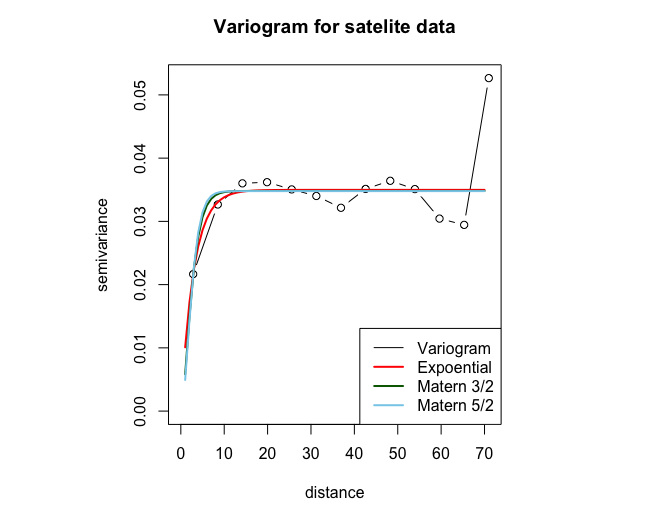
\includegraphics[width=1.4\linewidth]{figurer/variogram_covariancefunctions.png}
    \caption{Variogram given as input to the case.}
    \label{fig:variogram}
	\endminipage\hfill
	\minipage{0.45\textwidth}
  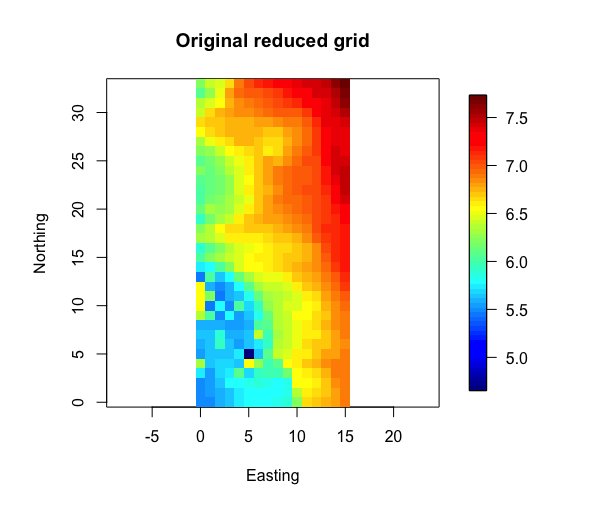
\includegraphics[width=1.4\linewidth]{figurer/original_reduced.png}
   \label{fig:original_data}
	 \caption{Actual data that are to be predicted on a reduced grid from the original.}
\endminipage
\end{figure}

\begin{figure}[p] 
\minipage{0.5\textwidth}
	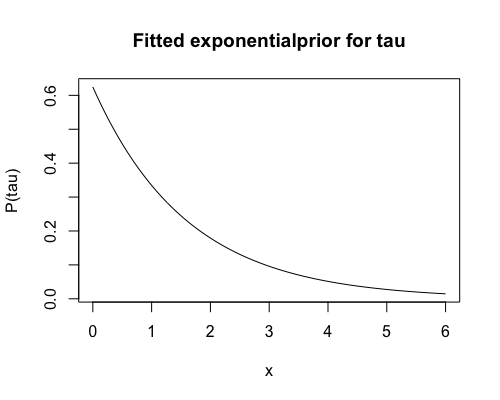
\includegraphics[width=1\linewidth]{figurer/fitted_exponential.png}
     \caption{Fitted prior distribution for $\tau$.}
     \label{fittedexponential}
	\endminipage\hfill
	\minipage{0.5\textwidth}
  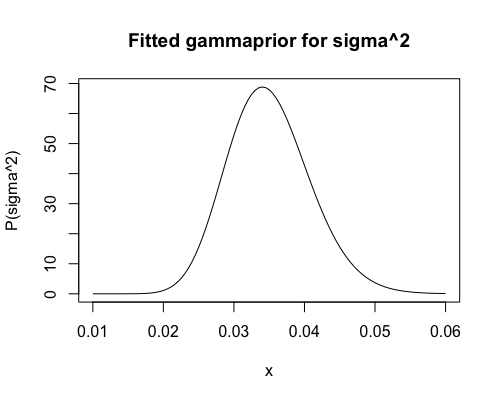
\includegraphics[width=1\linewidth]{figurer/fitted_gamma.png}
	 \caption{Fitted prior distribution for $\sigma^2$}
	 \label{fittedgamma}
\endminipage
\end{figure}

\subsubsection{Model specification and starting point of analysis} \label{subs:model}
As a necessary preliminary for the predictive analysis the temperature attribute of all the coordinates is modelled as a stochastic variable. Attaining a Gaussian process to describe trend and variability of model, the grid is viewed as a GRF. The connection between variables in this model will revolve around spatial location within the grid, where the trendfunction will be estimated by GLS regression on the sampled data. The covariance will be described by an isotropic, where results from all three covariancefunctions of (\ref{eq:covariance_functions}) will be presented individually. \\
The model process is fitted into the hierarchical model (HM) design described in (\ref{model:hm}). With $Y$ denoting the temperature variables at locations $\vec{s}$, that's set to be distributed according to the Gaussian process, the hierarchical model follows as
\begin{align*}
\begin{split}
\textbf{Data model: }& \vec{Z}(\vec{s}) = \vec{Y}(\vec{s}) + \vec{\epsilon}(\vec{s}), \quad \vec{\epsilon}(\vec{s}) \sim \mathcal{MVN} \big(\vec{0},\phi^2I(\vec{s}) \big) \\
\textbf{Process model: }& \vec{Y} = \vec{\mu} + \rho(\vec{s}), \quad \rho(\vec{s}) \sim \mathcal{MVN} \big(\vec{0}, \ C_Y(D(\vec{s}), \sigma^2, \tau ) \big) \\
\textbf{Prior model: }& \sigma^2 \sim \text{Gamma}(\alpha, \kappa), \quad \tau \sim \text{Exp}(\lambda)
\end{split}
\end{align*}
The intensity of the sampling noise, $\phi^2$, is the only one of the parameters that will be fixed. The motivation for doing so is that sampling noise may be viewed as more related to the equipment being used than the analysis in which it is included. Compared to the other parameters, one may have much more information about this parameter, as it may be stated by the equipment manufacturer or be tested separately in controlled environments. For the results, $\phi^2 = 0.2$ has been used. 

With the trend $\vec{\mu}$ is to be estimated by GLS on the sampled data eventually the data model is redefined as 
\begin{align} \label{eq:data_model}
\begin{split}
\textbf{Data model: }\vec{Z}(\vec{s}) &= X(\vec{s})\hat{\vec{\beta}} + \epsilon(\vec{s}) + \rho(\vec{s}) \\
\implies \vec{Z}(\vec{s}) &\sim \mathcal{MVN} \big( X(\vec{s})\hat{\vec{\beta}}, \ X(\vec{s}) \Sigma_{\hat{\beta}} X(\vec{s})^{T} + C_Y(D(\vec{s}), \sigma^2, \tau ) + \phi^2I(\vec{s}) \big)
\end{split}
\end{align}
where  Var${\hat{\beta}} = \Sigma_{\hat{\beta}} =  \bigg( X(\vec{s_0})^T \cdot \big( C_Y(D(\vec{s_0}), \sigma^2, \tau \big) + \phi^2I(\vec{s_0}) )^{-1} \cdot X(\vec{s_0}) \bigg)^{-1}$. \\

\subsection{Analysis}
\subsubsection{Choosing prior-parameters}
As a consequence of defining our model with prior-distributions for $\sigma^2$ and $\tau$, we must somehow estimate or choose parameters for their distributions. In order to do so, the variogram given as a part of the case preliminary has been utilized to estimate the GRF parameters of $\sigma^2$ and $\tau$. Given the three covariancefunctions in \ref{eq:covariance_functions}, the one may try to fit the the parameters of the chosen covariancefunction to the line. Denoting the discrete variogram values at points $k$ as $\gamma_k$ and the fitted covariancefunction at the same points as $\hat{\gamma}_k(\sigma^2, \tau)$, this is done by minimizing the associated lossfunction
\begin{equation} \label{eq:loss_function}
Loss(\sigma^2, \tau) = \sum_k \bigg( \frac{\gamma_k - \hat{\gamma}_k(\sigma^2, \tau)}{\gamma_k} \bigg)^2
\end{equation}
Notice that we only have two parameters to be estimated for each covariancefunction as the nugget effect has been assumed to be negligible, resulting in more stable computation of fit. This minimization has been performed using the \textit{variofit} function in the \textit{geoR} package found in the programming environement R. Obviously, the covariance functions are exponentially decaying as a function of distance with the three chosen in \ref{eq:covariance_functions}. In order to visually compare the fit, we use the relation between the variogram of a isotropic process and its covariancefunction that is
\begin{align} \label{eq:variogram_covariancefunction}
\begin{split}
    2\gamma(\textbf{s},\textbf{t}) &= Var(Y(\textbf{s}) - Y(\textbf{t})) \\
    &= Var(Y(\textbf{s})) + Var(Y(\textbf{t})) - 2Cov(Y(\textbf{s}),Y(\textbf{t})) \\
    \implies \gamma(\textbf{s},\textbf{t}) &= \sigma^2 - Cov(\|\textbf{s}-\textbf{t}\|)
\end{split}
\end{align}

The variogram is then overlain with fitted covariancefunctions, adapted by equation (\ref{eq:variogram_covariancefunction}), from \ref{eq:covariance_functions} in figure (\ref{fig:variogram}).  

Denoting the estimated values as $\hat{\sigma}^2$ and $\hat{\tau}$, one could have performed predictioning straight away. However, in an attempt to reduce the uncertainty in using this variogram, $\hat{\sigma}^2$ and $\hat{\tau}$ is used to fit parameters for the priors. This has been done by using a \textit{method of moments} inspired approach. As we have a single parameter prior for $\tau$, its mean and variance is estimated by 
\begin{align}
\hat{\lambda} = \frac{1}{\hat{\tau}}
\end{align}
With $\sigma^2$ given a gamma-prior, one needs to estimate two parameters. Denoting $\sum_k (\gamma_k - \hat{\sigma}^2)^2$ as $s_*^2$, the following approximation is used to set parameters $\alpha$ and $\beta$:
\begin{align}
\mathbf{E}(\sigma^2) = \frac{\alpha}{\beta} \approx \hat{\sigma}^2, \quad
\mathbf{Var}(\sigma^2) = \frac{\alpha}{\beta^2} \approx s_*^2 
\implies 
\hat{\alpha} = \frac{(\hat{\sigma}^2)^2}{s_*^2}, \quad  \hat{\beta} = \frac{\hat{\sigma}^2}{s_*^2}
\end{align}

The resulting prior-distributions are presented in figures (\ref{fittedexponential}) and (\ref{fittedgamma}).

\subsubsection{Discretizing the prior domains}
As the analysis relies on a numerical summation over the prior domains, a strategy must be defined to discretize the domains into $n_{\sigma^2}$ and $n_{\tau}$ divisions used the summation \ref{eq:expected_variance_grf_posterior}. In this case a method of \textit{stratified sampling} has been used. Given size-input $n_{\sigma^2}$, $(0,\inf)$ is subdivided into $n_{\sigma^2}$ divisions, each part corresponding to a $\frac{1}{n_{\sigma^2}}$ probability mass of the prior. Random samples are simulated until minimum one sample within each division is obtained. The same procedure is performed for $n_{\tau}$. 

The joined domain of $\tau$ and $\sigma^2$ is then considered a grid, with each cell corresponding to samples $(\tau_i, \sigma_j^2)$ having a probability mass of $\Delta_{ij} = \frac{1}{n_{\sigma^2} \cdot n_{\tau}}$ due to independence of priors. With both the normalizing constaHowever, may also be definedt and the summation for predictioThis progame discretization, all $\Delta_{ij}$ cancels as they are independent of $(\tau_i, \sigma_j^2)$ and are therefore omitted from the calculations. A disadvantage is obviously the problem of simulating random samples for all the divisions if the number of divisions become high. However, $n_{\tau}$ and $n_{\sigma^2}$ is kept relatively low in this case. 

\subsubsection{Results}	
Due to time-limitations, only a select predefined designs were used to produce results. The designs are presented in figure (\ref{fig:designs}). 

\begin{figure}[h]
	\hspace{-65pt}
	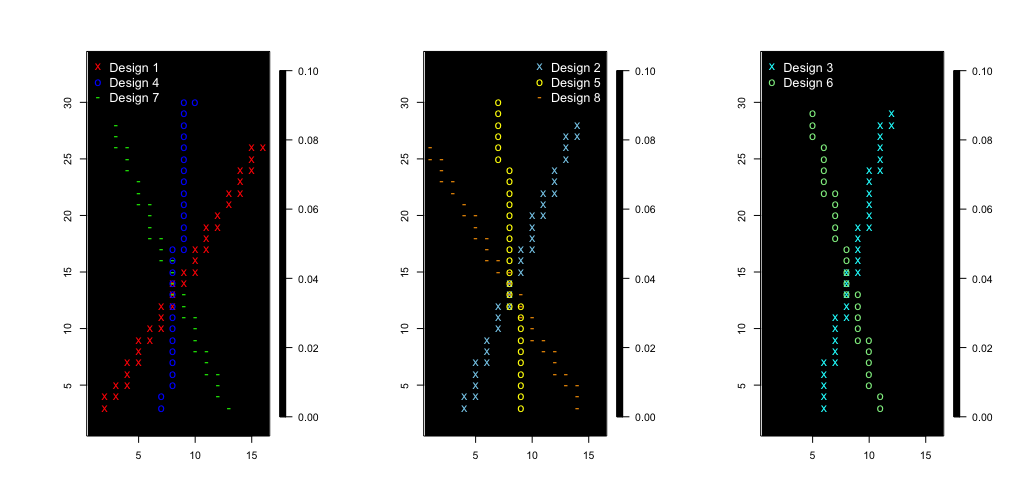
\includegraphics[width=1.3\linewidth]{figurer/design_lines.png}
    \caption{Sampling designs used to produce results.}
    \label{fig:designs}
\end{figure}

As the model is reliant on estimation of trend, an initial data sample has to be obtained. To estimate the spatially averaged predictive standard deviation, each design presented in figure (\ref{fig:designs}) was used as an initial design. Samples was obtained from this initial design, and possible new designs for further predictive analysis of the area was the remaining sample designs.

Using the procedure described in subsection (\ref{}), results are presented in table (\ref{tab:prior_parameters}). Each number signifies the estimated spatially averaged standard deviation from equation (\ref{eq:criteria}) by the various combinations. The design on top of the table signifies the initial path with realized values $Z$. The design at the left signifies the proposed added path in which we Monte Carlo simulate realizations $Z_a$ to use in equation (\ref{eq:criteria}). 

\newpage
\begin{figure}[!ht]
	\centering
	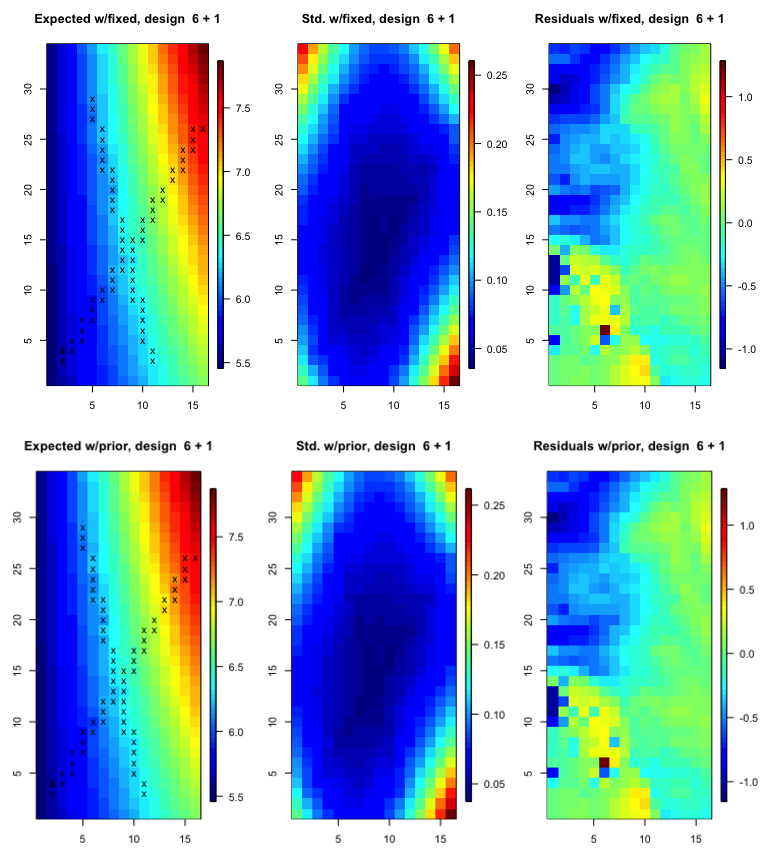
\includegraphics[width=0.6\linewidth]{figurer/final61.png}
    \caption{Prediction results for combined designs 6 + 1}
    \label{fig:results_61}
\end{figure}

\begin{figure}[!ht]
	\centering
	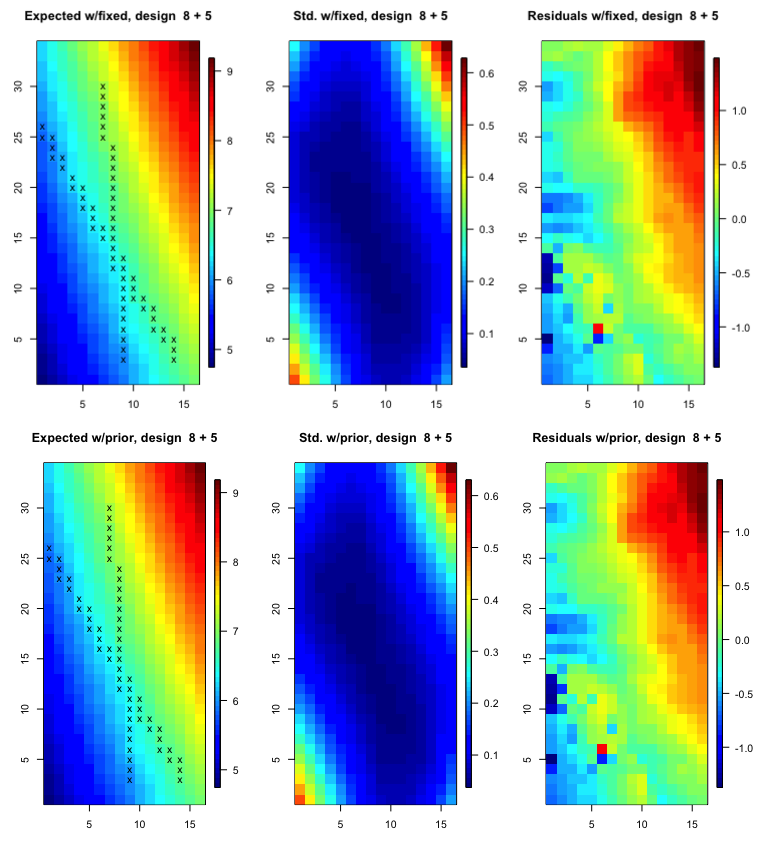
\includegraphics[width=0.6\linewidth]{figurer/final85.png}
    \caption{Prediction results for combined designs 8 + 5}
    \label{fig:results_85}
\end{figure}

\newpage

In these simulations, the measurement noise was set as $\phi^2 = 0.64$ and the Matern covariance function with $\nu = \frac{5}{2}$ was used. The prior discretization was performed with $n_{\sigma^2} = n_{\tau} = 10$ and yielded the following prior values: 
\begin{align*}
\begin{split}
\sigma^2 \in &\{0.02580851, 0.02883705, 0.03074835, 0.03233533, 0.03380639 \\ & \ 0.03527218, 0.03683043, 0.03861879, 0.04093687, 0.04503625 \} \\
\tau \in &\{0.02811741, 0.08908788, 0.15769846, 0.23614194, 0.32771585, \\ & \ 0.43771735, 0.57548019, 0.75992392, 1.03994281, 1.64216826 \}
\end{split}
\end{align*} 
Lastly, a total of 50 Monte Carlo samples was used to evaluate the criteria of m, spatially averaged standard deviation, for now denoted as SASD.\\

\begin{minipage}{\linewidth}
\captionof{table}{SASD with prior parameters} \label{tab:prior_parameters} 
\hspace{-35pt}
\begin{tabular}{ l || c | c | c | c | c | c | c | c } 
$Z_a$ \textbackslash  $Z$ & Design 1 & Design 2 & Design 3 & Design 4 & Design 5 & Design 6 & Design 7 & Design 8 \\
\hline \hline
Design 1 & - & 548.0111 & 490.2626 & 472.2716 & \textbf{465.4389} & \textbf{461.4315} & \textbf{458.3172} & \textbf{457.1136} \\
Design 2 & 548.0420 & - & 549.6023 & 490.1057 & 473.6499 & 465.6733 & 460.4351 & 458.5897 \\
Design 3 & 490.2403 & 549.4966 & - & 547.7782 & 495.0345 & 474.8508 & 464.7677 & 461.2044 \\
Design 4 & 472.3915 & 490.0712 & 547.8146 & - & 580.9237 & 498.8230 & 473.9019 & 466.1729 \\
Design 5 & 465.5245 & 473.6227 & 495.0963 & 580.9661 & - & 573.4793 & 495.3815 & 476.5188 \\
Design 6 & 461.4052 & 465.4790 & 474.7950 & 498.7048 & 573.4010 & - & 555.6704 & 495.8328 \\
Design 7 & 458.3496 & 460.5030 & 464.8691 & 473.9674 & 495.4149 & 555.7863 & - & 559.4372 \\
Design 8 & \textbf{457.1382} & \textbf{458.4126} & \textbf{461.1775} & \textbf{466.1601} & 476.5174 & 495.9166 & 559.3891 & -
\end{tabular}
\end{minipage}
\ \\

Evidently from the results, design 1 or design 8 are the ones prefered by our criteria, although only marginally in some cases. Based on the geometry of the design paths used in this analysis, this doesn't come as any surprise. As a note, the preferred addition to the existing path is seemingly the path that covered most of the area not included by the initial path. To assess the value of integrating the prior parameters out from the posterior distribution, the natural comparison are the same results with fixed parameters. In these simulations $\sigma^2 = 0.03486239$ and $\tau = 0.5481692$, which were the optimized values found by equation (\ref{eq:loss_function}) on the input-variogram. the results are found in table (\ref{tab:fixed_parameters}).

\begin{minipage}{\linewidth}
\captionof{table}{SASD with fixed parameters} \label{tab:fixed_parameters} 
\hspace{-35pt}
\begin{tabular}{ l || c | c | c | c | c | c | c | c } 
$Z_a$ \textbackslash  $Z$ & Design 1 & Design 2 & Design 3 & Design 4 & Design 5 & Design 6 & Design 7 & Design 8 \\ \hline \hline
Design 1 & - & 548.3832 & 490.2182 & 471.9795 & \textbf{464.9614} & \textbf{460.7763} & \textbf{457.5650} & \textbf{456.2909} \\
Design 2 & 548.3832 & - & 549.8854 & 490.0902 & 473.3898 & 465.1057 & 459.8781 & 457.8017 \\
Design 3 & 490.2182 & 549.8854 & - & 548.2868 & 495.0969 & 474.4967 & 464.3427 & 460.5580 \\
Design 4 & 471.9795 & 490.0902 & 548.2868 & - & 581.2475 & 498.6920 & 473.6160 & 465.6364 \\
Design 5 & 464.9614 & 473.3898 & 495.0969 & 581.2475 & - & 573.8424 & 495.4848 & 476.2670 \\
Design 6 & 460.7763 & 465.1057 & 474.4967 & 498.6920 & 573.8424 & - & 555.9909 & 495.9254 \\
Design 7 & 457.5650 & 459.8781 & 464.3427 & 473.6160 & 495.4848 & 555.9909 & - & 559.8999 \\
Design 8 & \textbf{456.2909} & \textbf{457.8017} & \textbf{460.5580} & \textbf{465.6364} & 476.2670 & 495.9254 & 559.8999 & -
\end{tabular}
\end{minipage}
\ \\
We see that the results coincide almost exactly as the simulations performed with prior distributions for the parameters $\sigma^2$ and $\tau$. As the results are similar for both simulations in terms of path design combinations, a measure was needed to see if the predictions produces different predictive results. Nooot

\subsubsection{Notes on computational cost}
An important aspect to consider when assessing these two methods used is the computational cost of using these methods. 

Integrating the parameters out by a numerical procedure is time-consuming due to the many matrix operations that are demanded in both GLS-estimation and evaluation of the multivariate Gaussian distribution. A quick analysis of the required calculations yields a running-time of $\mathcal{O}(n_{\tau} \cdot n_{\sigma^2} \cdot n_{grid size}^3 \cdot n_{Monte Carlo})$ for the model using prior parameters. Assuming a rectangular grid with dimensions $n_x \cdot n_y$ we get the running time as $\mathcal{O}(n_{\tau} \cdot n_{\tau} \cdot n_{x}^3 \cdot n_{y}^3\cdot n_{Monte Carlo})$ versus a $\mathcal{O}(n_{x}^3 \cdot n_{y}^3\cdot n_{Monte Carlo})$ for fixed parameters. Although the procedure for fixed parameter is quicker by some constantfactors, it would still be unacceptable in most cases when $n_{grid_size}$ becomes large. Based on the time used to derive the results in tables (\ref{tab:prior_parameters}) and (\ref{tab:prior_parameters}), I would characterize them as \textit{extremely slow} in the model with prior parameter and \textit{slow} despite the relatively small size of the gridded area. 

\subsection{Discussion}
By the results obtained in tables (\ref{tab:prior_parameters}) and (\ref{tab:fixed_parameters}), combined with ..., there's strong arguments for saying that the two models don't yield significant different results. When viewing the results, the effect of estimating the trend and how it affects the covariance of the latent process. As the trend has to be estimated, we introduce more variability into the model, perhaps in such a way that the GP-covariance "drowns" in the covariance introduced by estimating the trend by GLS. Evidently, this may be the case as the variogram gives a very low estimated $\sigma^2$, and is obviously the case when looking away from the sample paths as the standard deviation of examples such as figures (\ref{fig}) and (\ref{fig}) are much higher in some areas. The end result may be that the parameter $\sigma^2$ becomes of little importance.

Another possible explanation as to why the prior parameter model and fixed parameter model yielded the same results may be the fact that they were based on a variogram that is in essence a very accurate calculation. In that sense, assigning a prior model on the basis of this variogram could be interpreted as attaining too much variability to something that has in essence very little variability. 

The correlation parameter $\tau$ achieves a somewhat decent estimate, with an estimated correlation of $\approx 0.07$ at distance 3 in the Matern covariancefunction with $\nu=\frac{5}{2}$. However, this means that the covariance matrix of the latent GP is in reality quite sparse. This could be a motivation for redefining the model in some way to exploit this fact, as the cubic term in the computational running-time arises from the many inverses and determinants that has to be computed from the covariance matrix of the model. 

Looking back at the results, one has to evaluate the simulations that were performed as well. The discretization of the priorgrid for $\sigma^2$ and $\tau$ could be increased, the measurement noise could be varied, other covariancefunctions should have been tried out and especially the number of Monte Carlo samples obtained in the evaluation of the criteria. This was all neglected due to a combination of the computational cost of performing multiple simulations and how much time that was available. A possible tool would be to use parallellization of the computations as each Monte Carlo sample may be performed independently of any other. However, this doesn't solve the underlying problem as it won't change the immense running time of the calculations.

Another aspect that should have been altered in simulations is the number and variety of sample paths that were tested. At the very least more varied paths should have been tested, as to perhaps achieve more informative results. Given more time and effort, some sort of "path designer" could have been programmed, so as to construct proposals for paths that were probable to adhere to the criteria in equation (\ref{eq:criteria}).
